\chapter{Конструкция безвинтового подводного робота с внутренними роторами}\label{ch:ch3}

Основываясь на математической модели движения, конструкция робота должна соответствовать следующим требованиям:

\begin{itemize}
	\item Перпендикулярность роторов.
	\item Для создания максимального эффекта момент инерции роторов должен быть максимальным.
	\item Центр масс всей системы должен быть расположен максимально близко к геометрическому центру эллипсоида.
\end{itemize}

Для минимального отклонения центра масс от геометрического центра эллипсоида вместо каждого ротора будем использовать пару роторов. В каждой паре роторы должны быть равноудалены от центра эллипсоида и распологаться на осях эллипсоида.

\section{Описание конструкции безвинтового подводного робота с внутренними роторами}

Безвинтовой подводный робот является мобильным роботом в форме эллипсоида и представляет собой сборную конструкцию (рисунок \ref{constr_BPR}). Основой конструкции является оболочка 1 в форме эллипсоида, составленная из двух одинаковых половин 2, присоединенных друг к другу по экваториальной плоскости с помощью дискообразной перегородки – платформы 3. Размер эллипсоида по большей оси составляет 300 мм, по меньшей – 200 мм. Толщина оболочки (3 мм) и применяемый материал обеспечивают необходимую прочность при погружении и перемещении робота. Соединение полуоболочек и платформы обеспечивает герметичность внутренней полости.

\begin{figure}[h]
	\centering
	\includegraphics[width=0.9\linewidth]{constr_BPR.png}%
	\caption{Конструкция и корпусные элементы экспериментальной модели безвинтового подводного робота}
	\label{constr_BPR}
\end{figure}

Размещение узлов на платформе выполнено таким образом, чтобы в максимальной степени обеспечить симметричное расположение масс относительно геометрического центра тела, а также по возможности обеспечить минимальное отклонение центра масс от геометрического.

Внутри корпуса робота установлены три пары роторов (далее система роторов) таким образом, что оси роторов расположены под углом $90^\circ$ по отношению друг к другу. Ось одной из пар роторов направлена вдоль оси вращения эллипсоида, а две другие пары расположены в экваториальной плоскости. Обеспечение точного управляющего воздействия $\omega_k (t)$ осуществляется с помощью встроенных в приводы датчиков обратной связи (энкодеров). Система роторов подводного робота включает пару роторов большего размера 4, установленных симметрично относительно платформы 3 на одной общей оси, и двух других пар роторов меньшего размера 5, расположенных (по направлениям осей) перпендикулярно первой паре и перпендикулярно друг другу в экваториальной плоскости. Оси малых роторов выполнены отдельно для каждого маховика и установлены соосно на некотором расстоянии друг от друга. Малые роторы соединены кинематически попарно с помощью промежуточных (дополнительных) осей и зубчатых пар таким образом, что их вращение происходит также, как если бы они были на одной общей оси.

Характеристики безвинтового подводного робота с внутренними роторами разработанной конструкции представлены в таблице~\ref{tabCharBPR}.
% : масса оболочки: $2.923$ кг; момент инерции маховиков большего размера: $7.491\cdot10^{-4}$ кг$\cdot$м; масса маховиков большего размера: $0.903$ кг;	момент инерции маховиков меньшего размера: $0.491\cdot10-4$ кг$\cdot$м;	масса маховиков меньшего размера: $0.337$ кг.

\begin{table}[h]
	\centering
	\caption{Характеристики безвинтового подводного робота с внутренними роторами}\label{tabCharBPR}
	\begin{tabular}{|l|c|}
		\hline
		Масса оболочки	&	$2.923$ кг 	\\ \hline
		Масса большого ротора &	$0.903$ кг	\\ \hline
		Масса малого ротора &	$0.337$ кг \\ \hline
		Момент инерции большого ротора 	& $7.491\cdot10^{-4}$ кг$\cdot$м \\ \hline
		Момент инерции малого ротора &  $0.491\cdot10-4$ кг$\cdot$м\\ \hline
	\end{tabular}
\end{table}

Фотографии робота в сборе и без половины оболочки представлены на рисунке \ref{Photo_BPR}.

\begin{figure}[h]
	\centering
	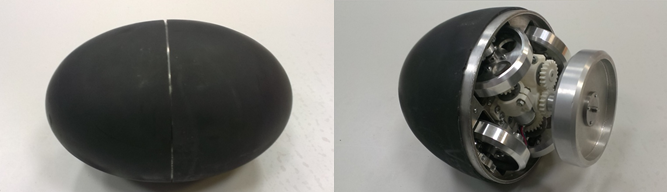
\includegraphics[width=0.9\linewidth]{Photo_BPR.png}%
	\caption{Фотографии безвинтового подводного робота}
	\label{Photo_BPR}
\end{figure}


Для приведения в движение системы роторов каждая из пар роторов оснащена высокомоментными мотор-редукторами, которые установлены в соответствующих опорах на платформе. Кинематическая схема передачи вращения от двигателей к роторам представлена на рисунке~\ref{KinemBPR}.

\begin{figure}[h]
	\centering
	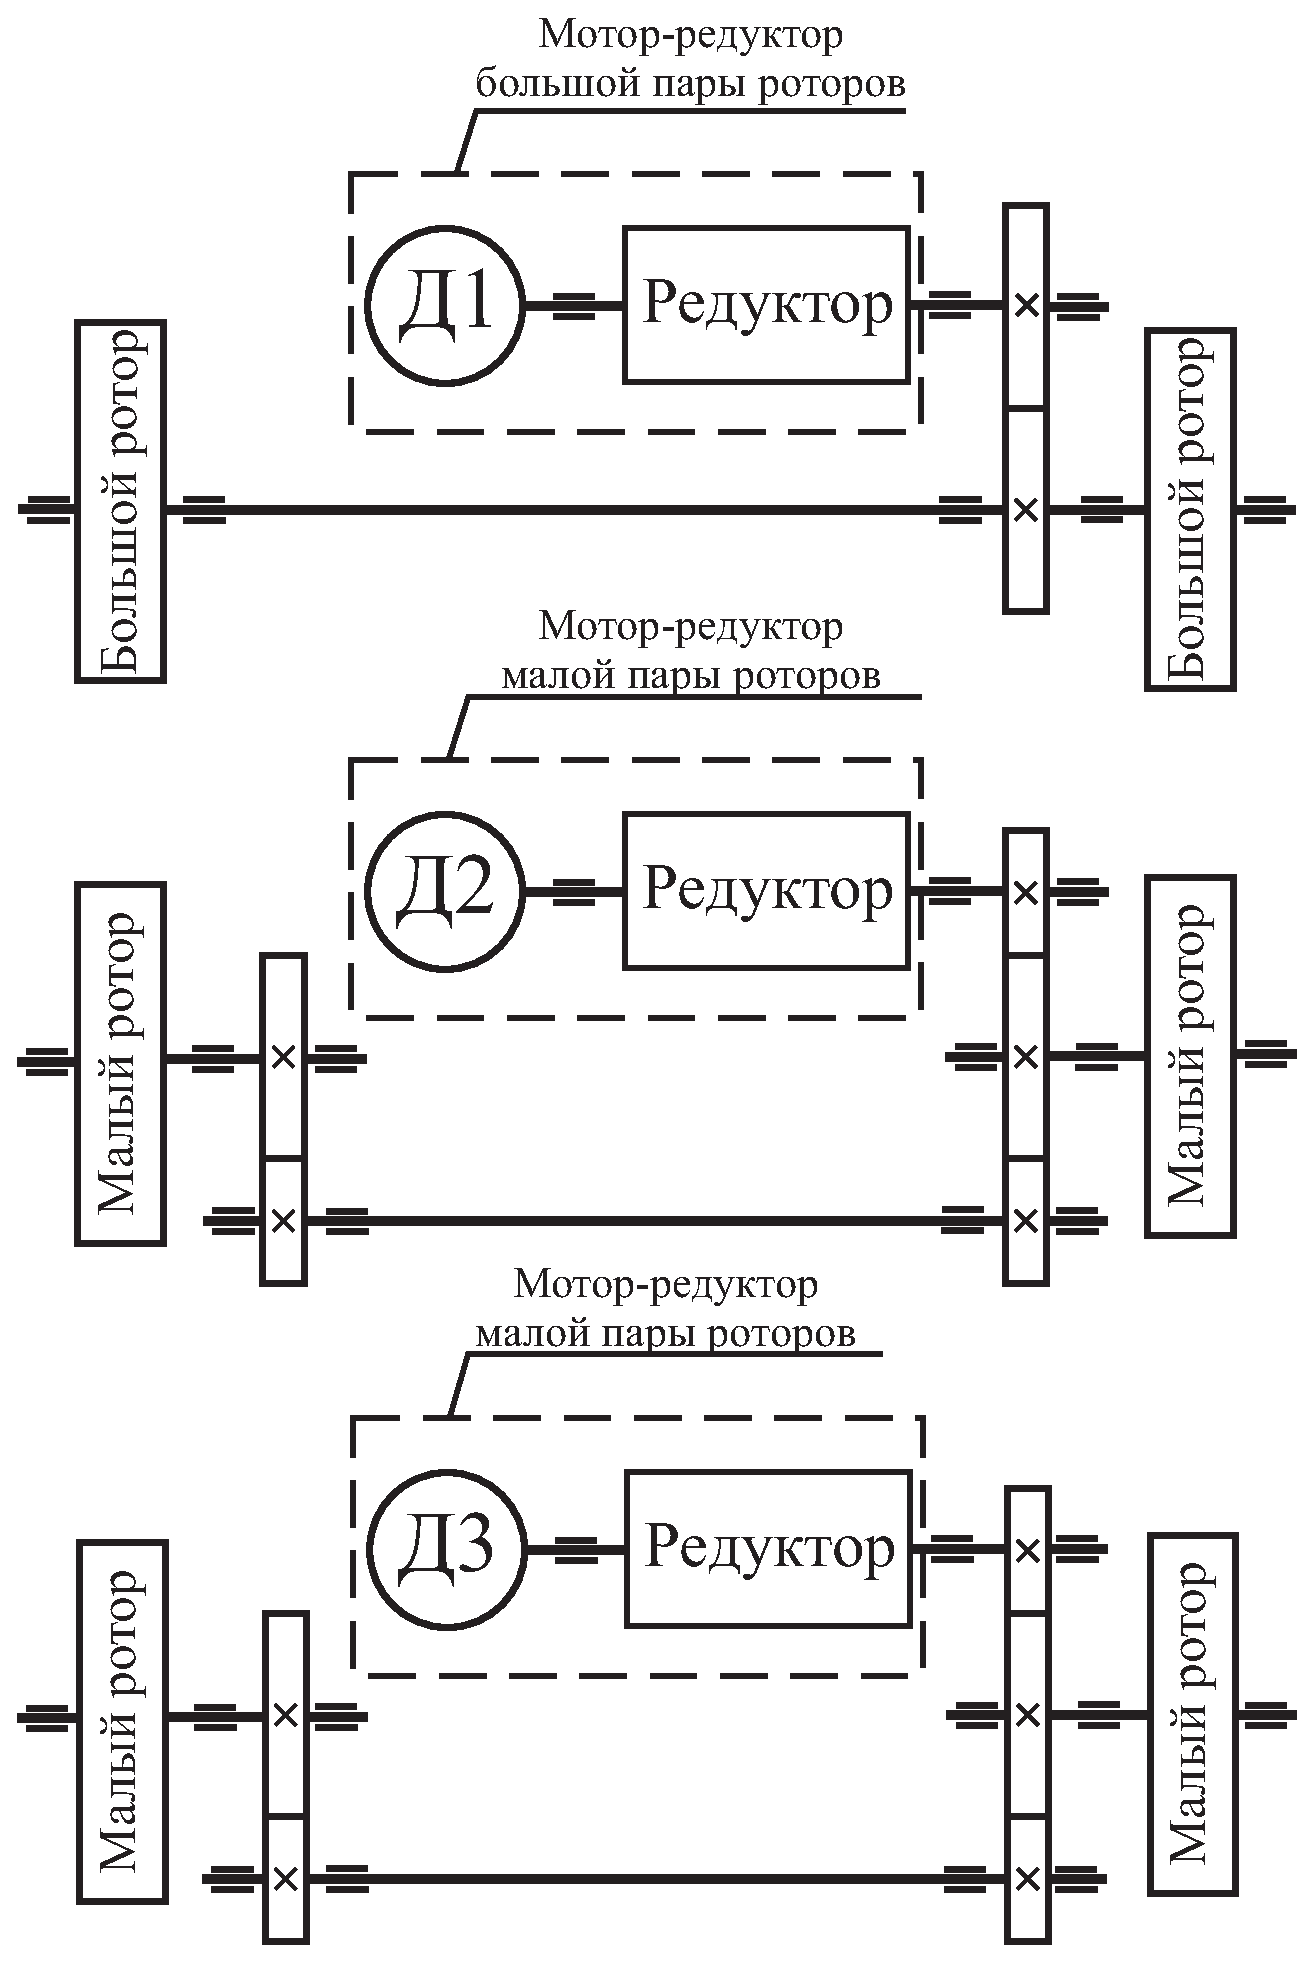
\includegraphics[width=0.6\linewidth]{KinemBPR.eps}%
	\caption{Кинематическая схема передачи вращения от двигателей к роторам}
	\label{KinemBPR}
\end{figure}

В качестве двигателя использовался мотор-редуктор фирмы Pololu с энкодером модели 25D Medium Power (см. рисунок~\ref{MotorBPR}). Характеристики двигателя: номинальное напряжение питания -- 12 В, передаточное отношение редуктора -- 47:1, момент на валу -- 0.6 Нм, максимальная скорость вращения -- 160 об/мин, ток холостого хода -- 200 мА, пусковой ток -- 2.1 А. 

\begin{figure}[h]
	\centering
	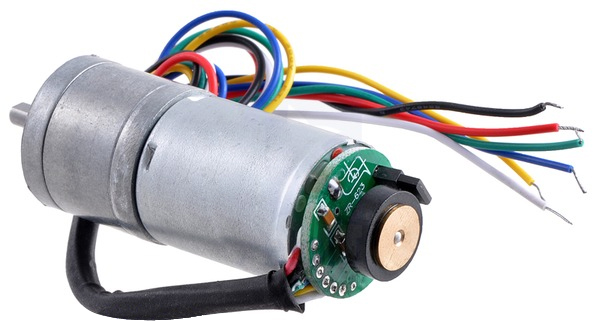
\includegraphics[width=0.5\linewidth]{Motor.jpg}%
	\caption{Мотор-редуктор фирмы Pololu с энкодером модели 25D Medium Power}
	\label{MotorBPR}
\end{figure}

Энкодер, расположенный на валу двигателя, использовался для определения положения ротора в течение экспериментов. Данный энкодер имеет специальный магнитный диск и датчики Холла, с помощью которых формируются сигнальные импульсы. Энкодер имеет два канала со смещением сигнала в четверть периода друг относительно друга, что позволяет определять направление вращения вала двигателя. Каждый канал формирует 12 импульсов на один оборот вала двигателя. Таким образом, используя два канала, считая переходы сигнала от низкого уровня к высокому и от высокого к низкому, можно получить 48 импульсов на один оборот вала двигателя. На микроконтроллере данные с энкодера обрабатываются таймером TIM1, который имеет специальный режим работы с энкодером (Encoder Mode), что позволяет аппаратно считать количество импульсов с двух каналов, учитывая направление вращения. 



Пара больших роторов расположена на оси, совпадающей с большей осью эллипсоида. Двигатель расположен параллельно этой оси и передача вращения от двигателя к роторам происходит через пару шестерен с 20 зубьями и передаточным отношением 1:1. 3Д-модель данной конструкции представлена на рисунке~\ref{BigRotorsBPR}.

\begin{figure}[h]
	\centering
	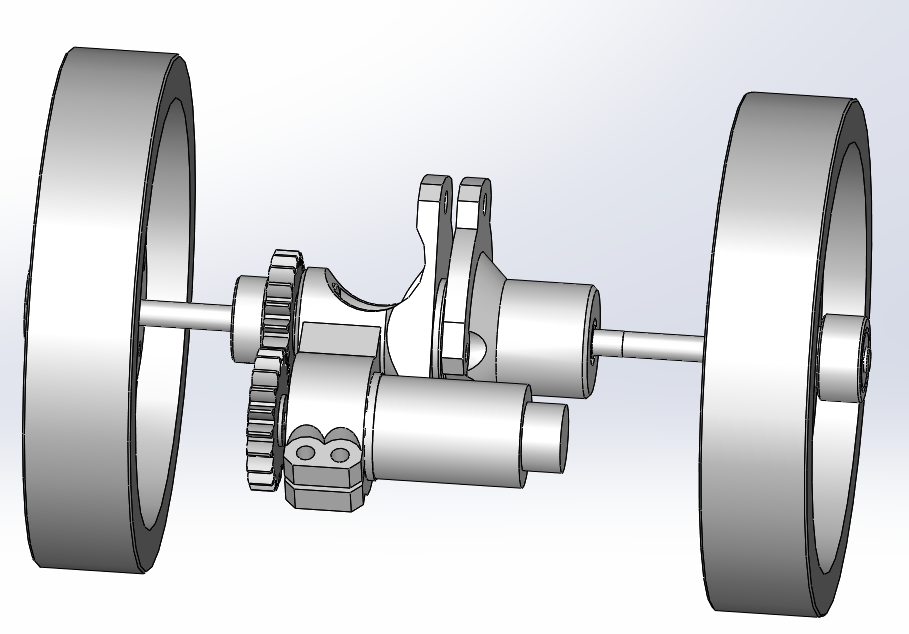
\includegraphics[width=0.6\linewidth]{BigRotorsBPR.png}%
	\caption{3Д-модель конструкции для передачи вращения от двигателя к паре больших роторов}
	\label{BigRotorsBPR}
\end{figure}

Для передачи вращения от двигателей к малым роторам используются промежуточные оси и шестерни на 12 и 20 зубьев (см. рисунок~\ref{KinemBPR}). Передаточное отношение между двигателем и каждым малым ротором составляет 1.6:1. 3Д-модель конструкции для передачи вращения от двигателя к одной паре малых роторов представлена на рисунке~\ref{SmallRotorsBPR}. Для второй пары малых роторов конструкция передачи вращения аналогичная.

\begin{figure}[!ht]
	\begin{minipage}[h]{0.5\linewidth}
		\center{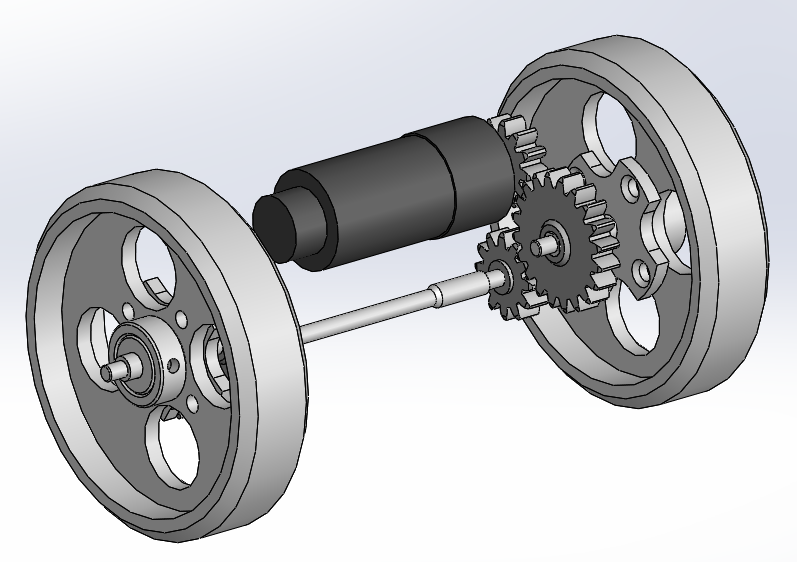
\includegraphics[width=0.8\linewidth]{SmallRotorsBPR1.png} \\ }
	\end{minipage}
	\hfill
	\begin{minipage}[h]{0.5\linewidth}
		\center{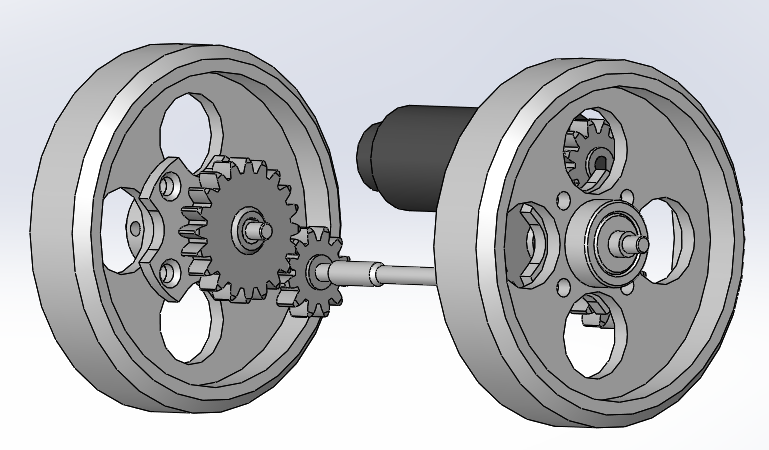
\includegraphics[width=0.9\linewidth]{SmallRotorsBPR2.png} \\ }
	\end{minipage}
	\caption{3Д-модель конструкции для передачи вращения от двигателя к паре малых роторов}
	\label{SmallRotorsBPR}
\end{figure}

На рисунке~\ref{SmallRotorsBPR3} представлено расположение двух пар малых роторов с их двигателями и элементами для передачи вращения. На рисунке~\ref{AllRotorsBPR} представлено взаимное расположение всех роторов робота.

\begin{figure}[h]
	\centering
	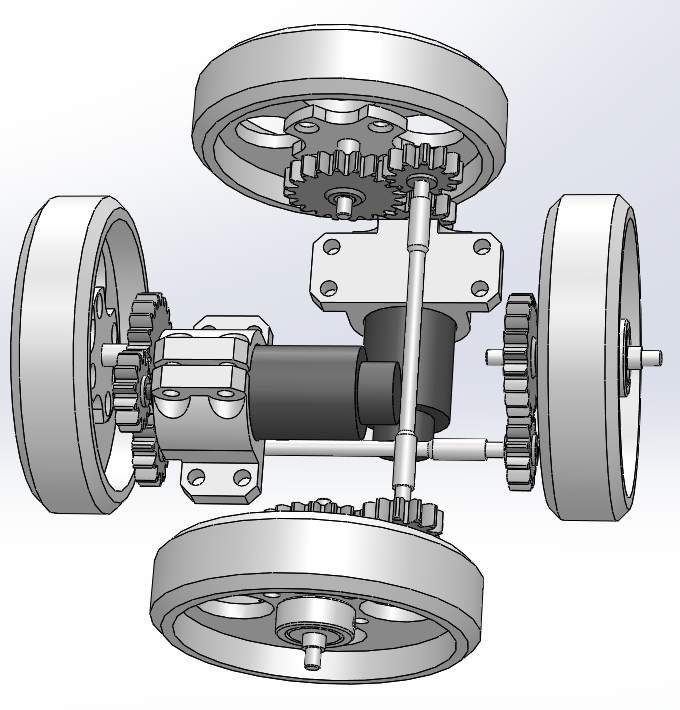
\includegraphics[width=0.6\linewidth]{SmallRotorsBPR3.png}%
	\caption{3Д-модель конструкции двух пар малых роторов с их двигателями и элементами для передачи вращения}
	\label{SmallRotorsBPR3}
\end{figure}

\begin{figure}[h]
	\centering
	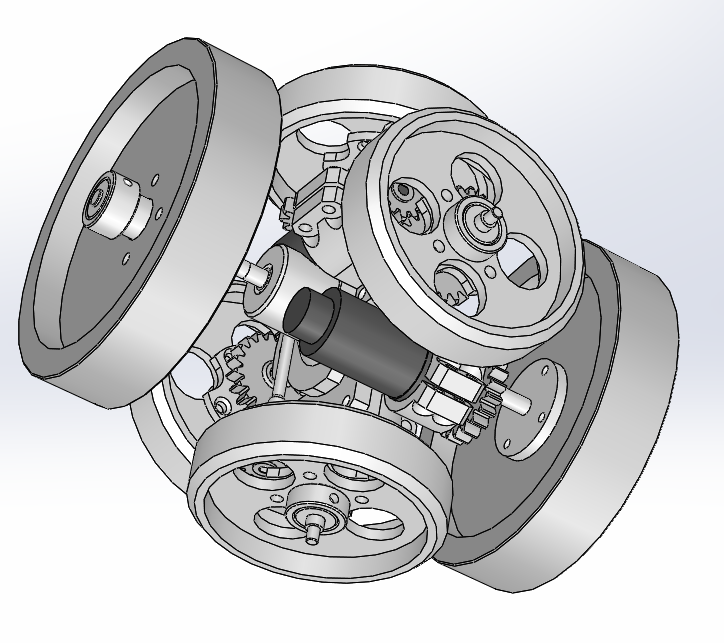
\includegraphics[width=0.6\linewidth]{AllRotorsBPR.png}%
	\caption{3Д-модель конструкции внутренних роторов безвинтового подводного робота}
	\label{AllRotorsBPR}
\end{figure}



В пространствах между большими и малыми роторами симметрично с двух сторон относительно платформы на панелях смонтированы модули питания 6, управления и связи.

В качестве модуля питания используется пара литий-полимерных (Li-Po) аккумуляторных батарей фирмы nVision (см. рисунок~\ref{Accum}) с номинальным напряжением 7.4 Вольта, емкостью 450 мАЧ и максимальным выходным током до 13.5 Ампер. Аккумуляторные батареи соединены друг с другом параллельно.

\begin{figure}[h]
	\centering
	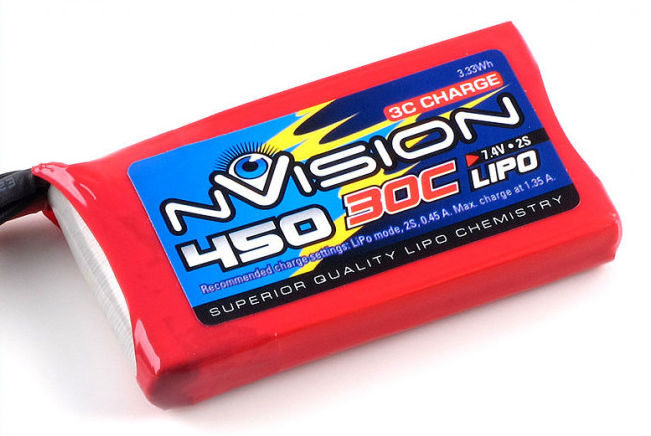
\includegraphics[width=0.6\linewidth]{Accum.png}%
	\caption{Аккумуляторная батарея фирмы nVision}
	\label{Accum}
\end{figure}


Передача данных для управления движением и получением дополнительной информации о состоянии системы может осуществляться по проводному и беспроводному вариантам связи. Проводной способ связи реализован с помощью переходника USB-USART на основе микросхемы CP2102, который, подключаясь к USB-разъему на персональном компьютере, позволяет создать виртуальный COM-порт. На микроконтроллере соответствующие выводы данного переходника подключены к выводам микроконтроллера, аппаратно поддерживающим интерфейс USART. Беспроводной вариант связи реализован с помощью bluetooth-модуля HC-06, который работает аналогичным образом переходнику USB-USART: с микроконтроллером модуль НС-06 взаимодействует посредством интерфейса USART, а с компьютером bluetooth-модуль соединяется, используя профиль SPP (Serial Port Profile), что также позволяет создать виртуальный СОМ-порт и работать с ним. Внешний вид переходника USB-USART и bluetooth-модуля HC-06 представлен на рисунке~\ref{uartModules}.

\begin{figure}[!ht]
	\begin{minipage}[h]{0.5\linewidth}
		\center{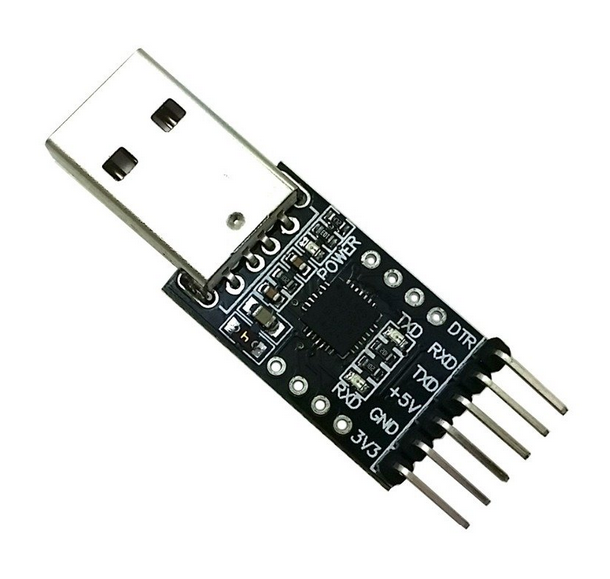
\includegraphics[height=0.7\linewidth]{Cp2102.png} }
	\end{minipage}
	\hfill
	\begin{minipage}[h]{0.5\linewidth}
		\center{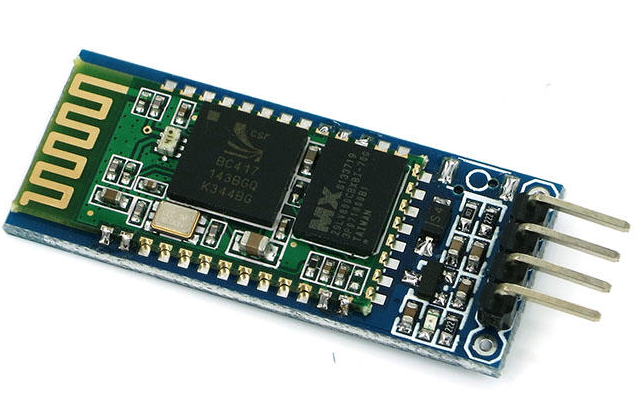
\includegraphics[height=0.6\linewidth]{HC-06.png} }
	\end{minipage}

	\begin{minipage}[h]{0.5\linewidth}
		\center{а}
	\end{minipage}
	\hfill
	\begin{minipage}[h]{0.5\linewidth}
		\center{б}
	\end{minipage}

	\caption{а) Модуль-переходник USB-USART. б) Bluetooth-модуль HC-06}
	\label{uartModules}
\end{figure}



Для погружения робот оснащен механизмом регулировки плавучести. Он состоит из двух одинаковых модулей плавучести 7, размещенных и закрепленных внутри полуоболочек в наиболее удаленных частях относительно платформы. Модули плавучести имеют в своем составе лопастной насос 8 с приводом 9 на основе микроэлектродвигателя с редуктором. Полости насоса --- воздушная и жидкостная имеют каналы 10, соединяющие их соответственно с внутренней полостью и внешней средой.

Для контроля глубины робот оснащен двумя датчиками давления MPX5010GP фирмы NXP (см. рисунок~\ref{PressureSensor}), расположенными рядом с модулями плавучести. Датчик является аналоговым, максимальная величина измеряемого давления -- 10 кПа, что соотвествует 1019.78 мм глубины погружения в воде. Датчик подключается к входу 12-битного аналого-цифрового преобразователя (АЦП) микроконтроллера. Характеристики датчика представлены в таблице~\ref{tabPressure}.

\begin{figure}[h]
	\centering
	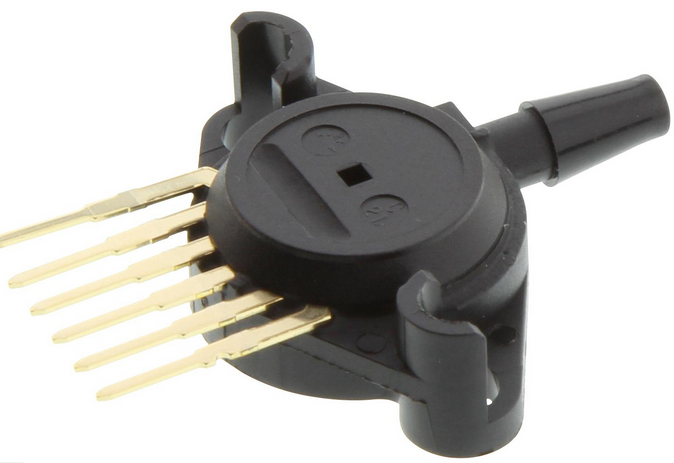
\includegraphics[width=0.5\linewidth]{PressureSensor.png}%
	\caption{Датчик давления MPX5010GP фирмы NXP}
	\label{PressureSensor}
\end{figure}

\begin{table}[h]
	\centering
	\caption{Характеристики датчика давления MPX5010GP фирмы NXP}\label{tabPressure}
	\begin{tabular}{|l|c|}
		\hline
		Максимальное рабочее давление	&	10 кПа 	\\ \hline
		Тмакс	&	125$^\circ$ C 	\\ \hline
		Тмин 	&	-40$^\circ$ C \\ \hline
		Время отклика 	& 1 мс \\ \hline
		Выходное напряжение при максимальном давлении	&  4.59 В\\ \hline
		Предельно допустимое давление & 40 кПа \\ \hline
		Напряжение питания 	& 5 Вольт\\ \hline	
		Потребляемый ток	& 5...10 мА\\ \hline	
		Точность	& 5\% \\ \hline
		Чувствительность в жидкости	& 4.413 мВ/мм \\ \hline
	\end{tabular}
\end{table}

Рассчитаем минимальное изменение глубины, которые может воспринимать датчик давления. Так как опорное напряжение АЦП микроконтроллера -- 3.3 Вольта, для преобразования выходного сигнала датчика, имеющего максимальное значение в 4.7 вольта, использовался делитель напряжения на резисторах номиналом 10 кОм и 15 кОм. Коэффициент преобразования данного делителя напряжения -- 1.67, а максимальное напряжение на АЦП микроконтроллера составило 2.81 В. АЦП, к которому подключены датчики давления является 12-ти разрядным с опорным напряжением 3.3 В. Поэтому разрешающая способность данного АЦП -- 3.2 мВ, а до делителя напряжения 5.12 мВ. Таким образом, можно определять изменение глубины на 1.16 мм.




Для определения ориентации робот имеет датчик на основе микросхемы MPU9250 (см. рисунок~\ref{Mpu9250}), который включает в себя трехосевой акселерометр, трехосевой гироскоп и трехосевой магнитометр. Данный датчик является цифровым, имеет на борту 16-битный аналого-цифровой преобразователь для оцифровки данных с датчиков. Датчик может быть подключен к микроконтроллеру по интерфейсам SPI или I2C. Характеристики датчика представлены в таблице~\ref{tabMpu}.

\begin{figure}[h]
	\centering
	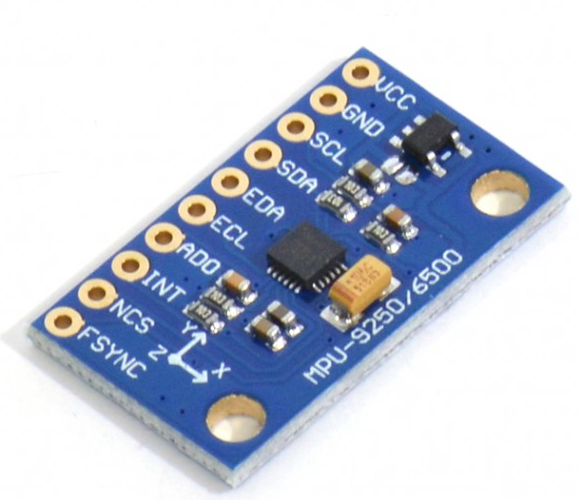
\includegraphics[width=0.3\linewidth]{Mpu9250.png}%
	\caption{Датчик MPU9250}
	\label{Mpu9250}
\end{figure}

\begin{table}[h]
	\centering
	\caption{Характеристики датчика MPU9250}\label{tabMpu}
	\begin{tabular}{|l|c|}
		\hline
		Тмакс	&	125$^\circ$ C 	\\ \hline
		Тмин 	&	-40$^\circ$ C \\ \hline
		Рабочие диапазоны гироскопа & ±250, ±500, ±1000, ±2000 $^\circ$/с \\ \hline
		Чувствительность гироскопа & 131, 65.5, 32.8, 16.4 LSB/$^\circ$/c \\ \hline
		Рабочие диапазоны акселерометра & ±2, ±4, ±8, ±16 g\\ \hline
		Рабочий диапазон магнитометра & ±4800 мкТл\\ \hline
		Напряжение питания & 2.4-3.6 В\\ \hline
		Рабочий ток гироскопа & 3.2 мА\\ \hline
		Рабочий ток акселерометра & 450 мкА\\ \hline
		Рабочий ток магнитометра & 280 мкА\\ \hline
		Ток в режиме сна & 16 мкА \\ \hline
	\end{tabular}
\end{table}

Для расчёта ориентации объекта в пространстве по показаниям датчиков акселерометра, гироскопа и магнитометра использовался фильтр Маджвика (Madgwick filter)~\cite{Madgwick}. Данный фильтр имеет две разновидности: IMU -- берет в  расчет данные с акселерометра и гироскопа, MARG -- учитывает данные с гироскопа, акселерометра и магнитометра. Фильтр MARG учитывает магнитные искажения и компенсирует смещения гироскопа. Ны выходе фильтра получаем кватернион, который описывает вращение объекта вокруг произвольной оси. Кватернион можно преобразовать в углы Эйлера, которые определяют углы крена, тангажа и рысканья. 

Точность определения углов ориентации объекта: 0.6$^\circ$ -- среднеквадратичное отклонение в неподвижном состоянии;
0.8$^\circ$ -- среднеквадратичное отклонение в подвижном состоянии.

На каждое обновление фильтра MARG необходимо выполнить 277 простых арифметических операций. Данный фильтр можно использовать с частотой обновления от 10 Гц. Из-за невысокой вычислительной нагрузки и возможности работать на низких частотах дискретизации данный фильтр подходит для вычисления углов ориентации на микроконтроллере. 





\section{Описание системы управления безвинтового подводного робота с внутренними роторами}

В полученных математических моделях управление роторами задается в виде вектора внутреннего гиростатического момента $\bK$. Для управления отдельным двигателем разработана следующая схема (см. рисунок \ref{Control_system}).

\begin{figure}[h]
	\centering
	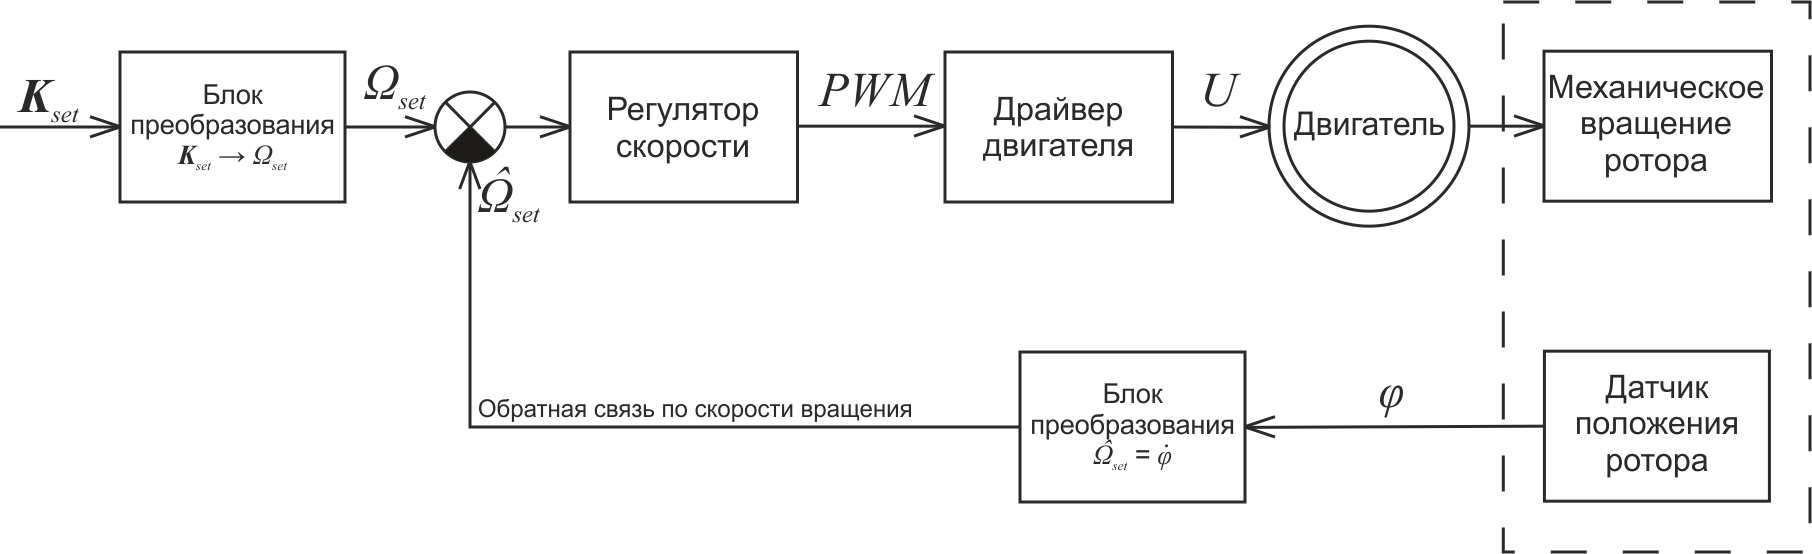
\includegraphics[width=0.9\linewidth]{Control_system.png}%
	\caption{Схема управления отдельным двигателем, где $\bK_{set}$ -- вектор внутреннего гиростатического момента; $\bOm_{set}$ -- угловая скорость вращения двигателя; $\hat{\bOm}_{set}$ -- фактическая скорость вращения двигателя; $PWM$ -- широтно-импульсная модуляция, рассчитаная для заданной скорости вращения; $U$ -- напряжение, подаваемое на двигатель; $\varphi$ -- фактическое положение ротора}
	\label{Control_system}
\end{figure}

Структурная схема системы управления безвинтового подводного робота, представлена на рисунке \ref{str_scheme}.

\begin{figure}[h!]
	\begin{center}
		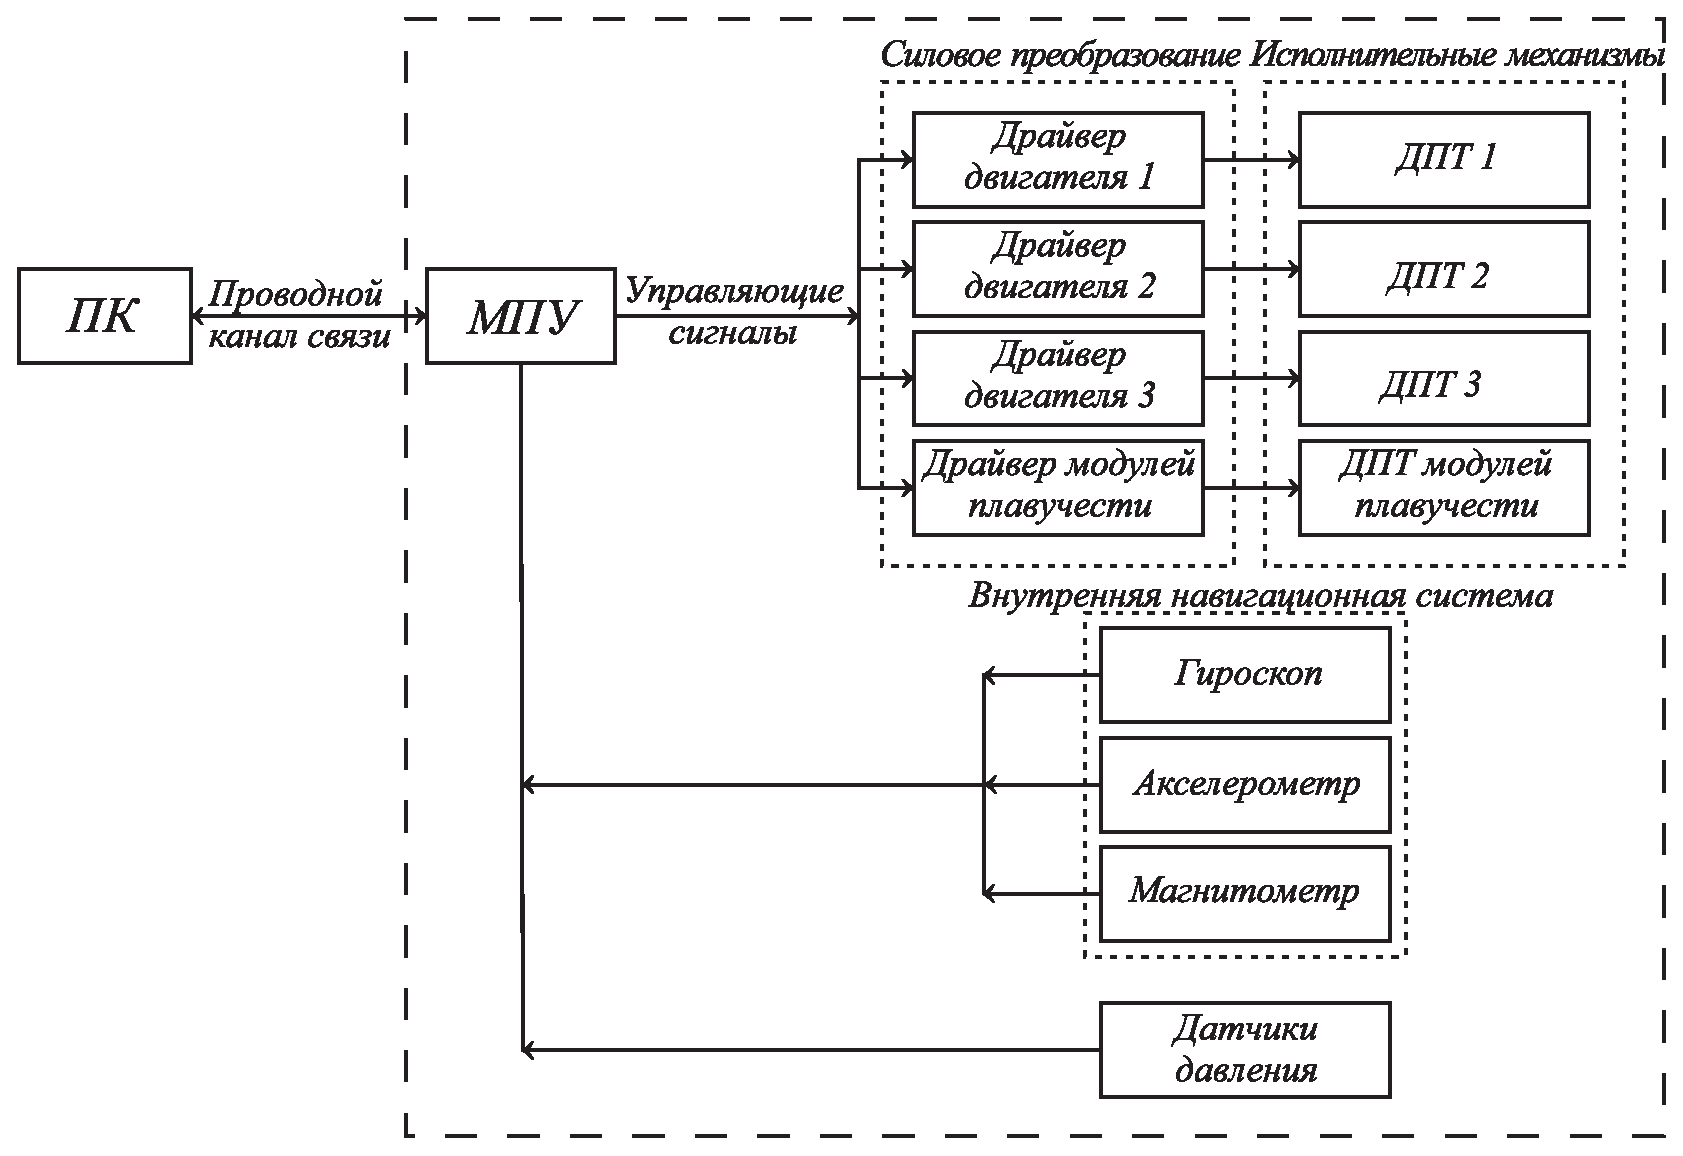
\includegraphics[width=0.8\linewidth]{StrSchemeBPR.eps}
		\caption{Структурная схема системы управления подводным роботом} \label{str_scheme}
	\end{center}
\end{figure}

Оператор на персональном компьютере (ПК, см. рисунок \ref{str_scheme}) задает команды управления подводным роботом. Команды передаются на микропроцессорное устройство (МПУ) по проводному или безпроводному (если робот находится на поверхности воды) каналу связи и представляют собой закодированные скорости вращения роторов или двигателей модулей плавучести. Далее микропроцессор обрабатывает полученные данные и формирует управляющий сигнал, подаваемый на драйверы двигателей или драйверы модулей плавучести, которые, в свою очередь, подают напряжение нужной формы и амплитуды на двигатели постоянного тока (ДПТ) или модули плавучести. Плата управления также содержит трехосевые акселерометр, гироскоп и магнитометр, которые являются внутренней навигационной системой робота и служат для определения ориентации робота. В качестве датчиков глубины погружения робота, используются датчики давления, расположенные в полюсах эллипсоида. Использование информации с данных датчиков в качестве обратной связи позволит регулировать плавучесть на заданной глубине погружения.


Система управления основана на микроконтроллере LPC1768. Плата управления с электронными компонентами, разработанная для робота представлена на рисунке~\ref{PCB_BPR}

\begin{figure}[h!]
	\begin{center}
		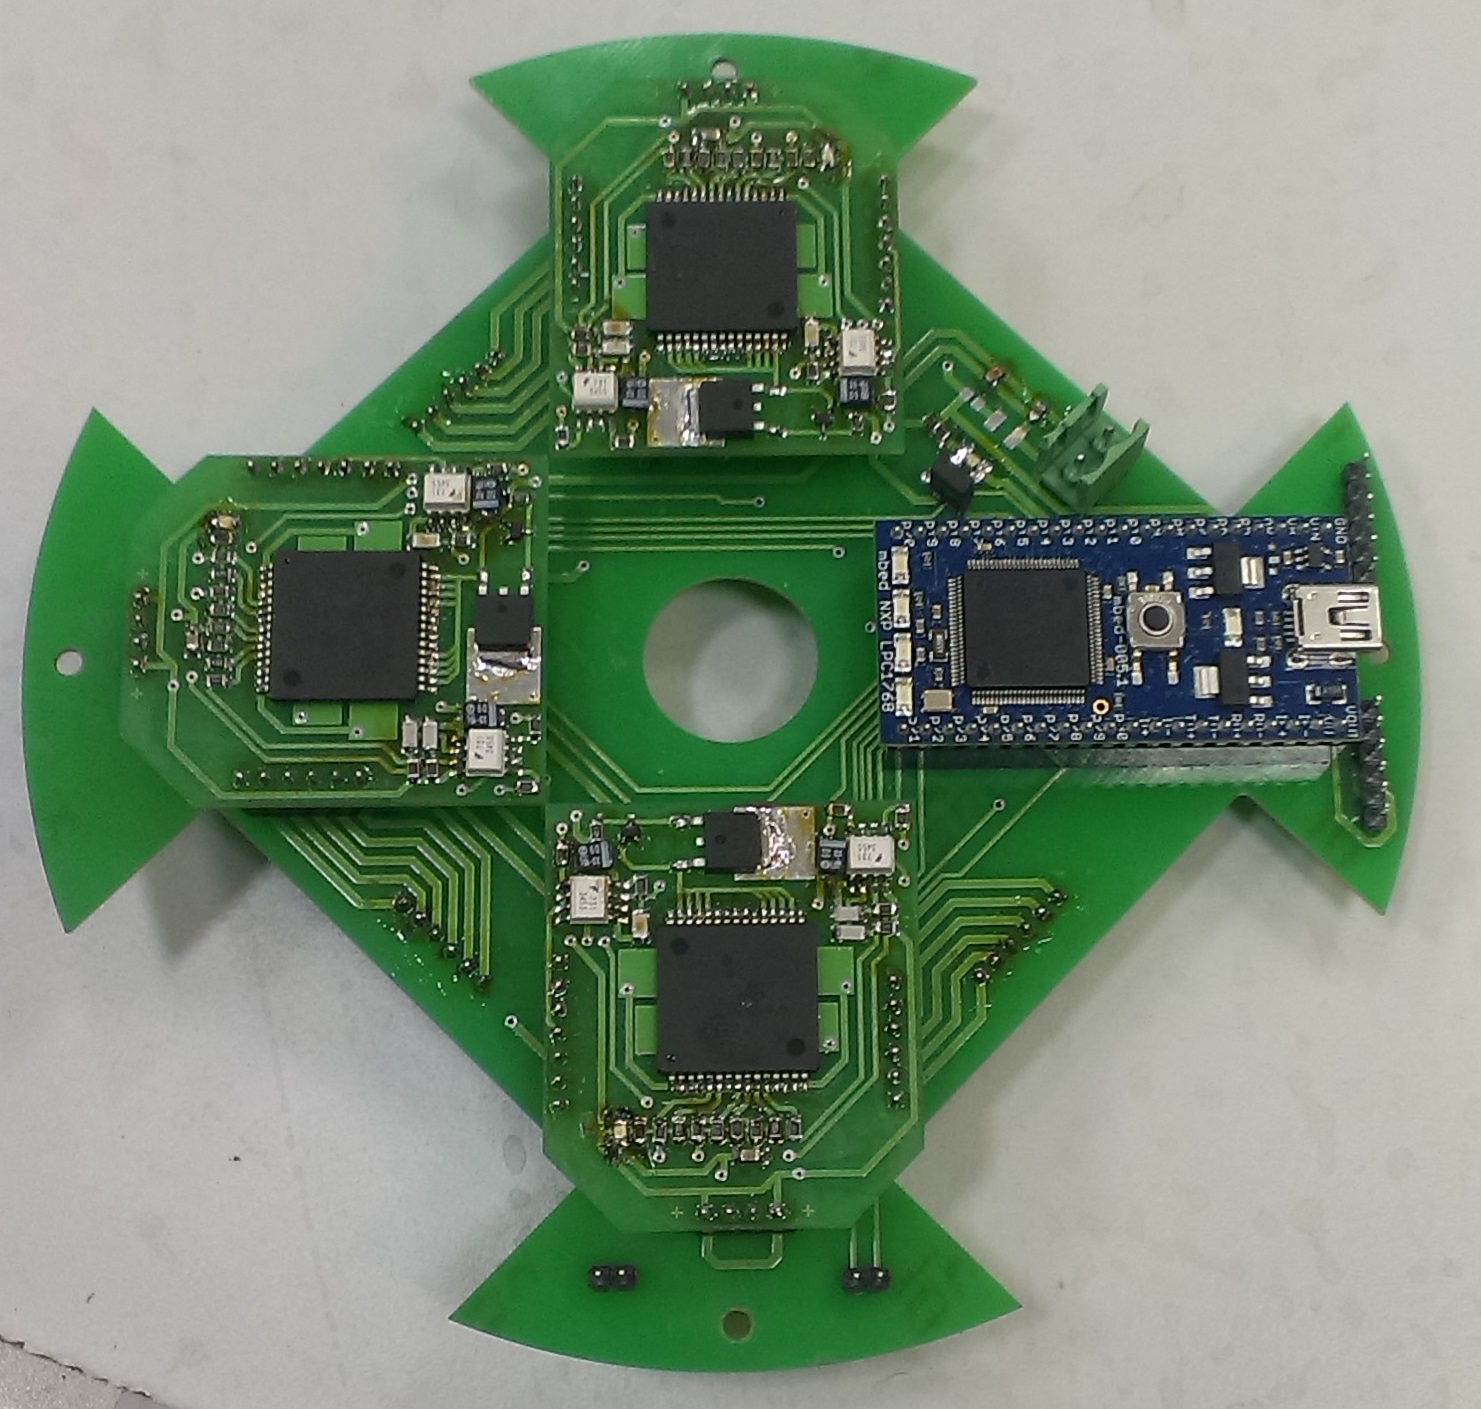
\includegraphics[width=0.8\linewidth]{PCB_BPR.png}
		\caption{Плата управления безвинтового подводного робота} \label{PCB_BPR}
	\end{center}
\end{figure}

Управление осуществляется с персонального компьютера (ПК), для которого было разработано специальное программное обеспечение. Для управления роботом необходимо задать направления и скорости вращения каждого из роторов, а также время разгона до заданной скорости. Отдельно осуществляется управление модулями плавучести, которые отвечают за погружение робота.



\clearpage